% !TEX root = ThesisGchatzi.tex

\section{Methods} 
\label{sec:knn_methods}

\graphicspath{{Papers/SpringerJournalOfBigData/}}

This section outlines the design and implementation of FML-$k$NN. One of the main contributions of FML-$k$NN is the unification of the three different processing stages into a single Flink session. Multi-session implementations, regardless of the distributed platform on which they are developed and operated, are significantly inefficient due to the following reasons:

\begin{itemize}
	\item \textbf{Multiple initializations of the distributed environment}: They increase the total wall-clock time needed by an application in order to produce the final results.
	\item \textbf{Extra I/O operations during each stage}: They introduce latency due to I/O operations and occupy extra HDFS space.
\end{itemize}

We avoid the above issues by unifying the distributed sessions into a single one. Figure~\ref{figure2} illustrates the unified session. The stages are executed sequentially and I/O operations on HDFS take place only during the start and end of the execution.

\begin{figure}[!ht]
	\centering
	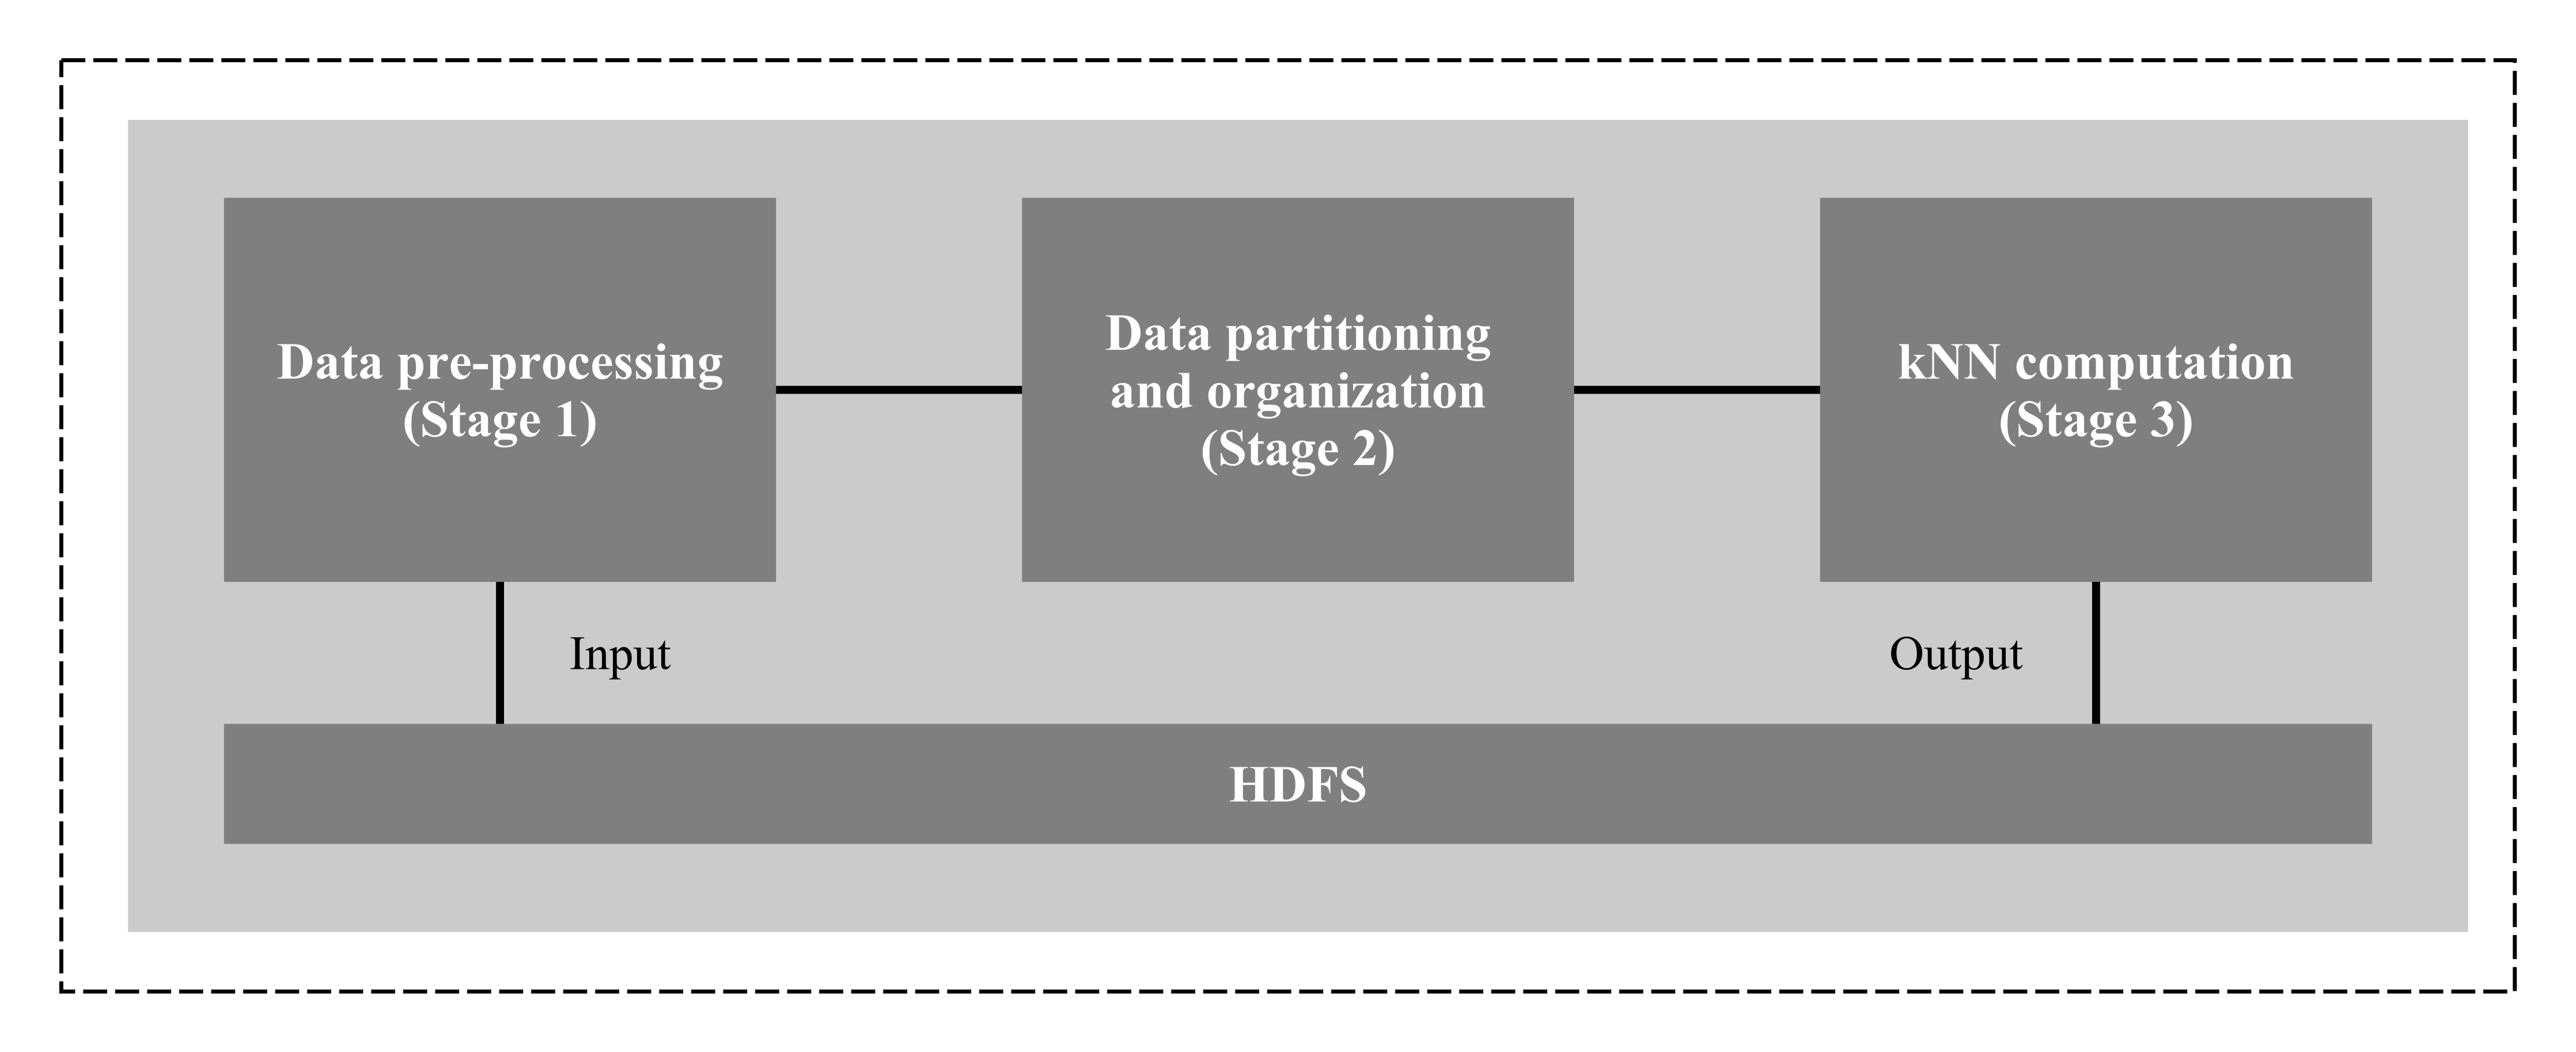
\includegraphics[width=0.9\textwidth]{figures/figure2.png}
	\caption{Single Flink session.}
	\label{figure2}
\end{figure}

\subsection{Dimensionality reduction and shifting}
The input dataset is consisted of points in a $d$-dimensional space. To perform dimensionality reduction, we transform each point into SFC values via either $z$-order, Gray-code, or Hilbert curve. By taking a closer look on the way the SFCs fill a two-dimensional space from the smallest value to the largest, one could easily notice that some elements are falsely calculated being closer than others, as the curve scans them first. This can have a negative impact on the result’s accuracy. 

To diminish the negative effect of such false approximations, we generate a pre-determined number of alternate versions of the dataset, where each element is randomly shifted by a pre-calculated random vector. As an example, let us suppose that we have a dataset whose elements consists of three features and a random vector $v=\{3, 5, 2\}$. Then, all the elements of the dataset are shifted using this vector, e.g., an element $el=\{2, 6, 9\}$ will be altered to $el'=\{2+3, 5+6, 2+9\}=\{5, 11, 11\}$. This is demonstrated for $z$-order curve in Figure 3, where the four bottom-left elements are shifted twice in the $x$-axis and once in the $y$-axis, altering the sequence in which they are scanned by the curve. This way, neighboring points that are distant on the curve will possibly be closer in the shifted dataset. This procedure compensates the lost accuracy, as it enables scanning the space in an altered sequence. During execution, the shifted dataset is concatenated with the original one and the algorithm is executed, producing \textit{multiple} groups of $k$NNs, from which the final $k$NNs are determined. The limitation of this approach is the fact that the size of the input dataset is increased according to the number of shifts $i\in{[1, \alpha]}$, where $\alpha$ is the total number of shifts. Finally, we should mention that the above process is similar for all SFCs.

\begin{figure}[!ht]
	\centering
	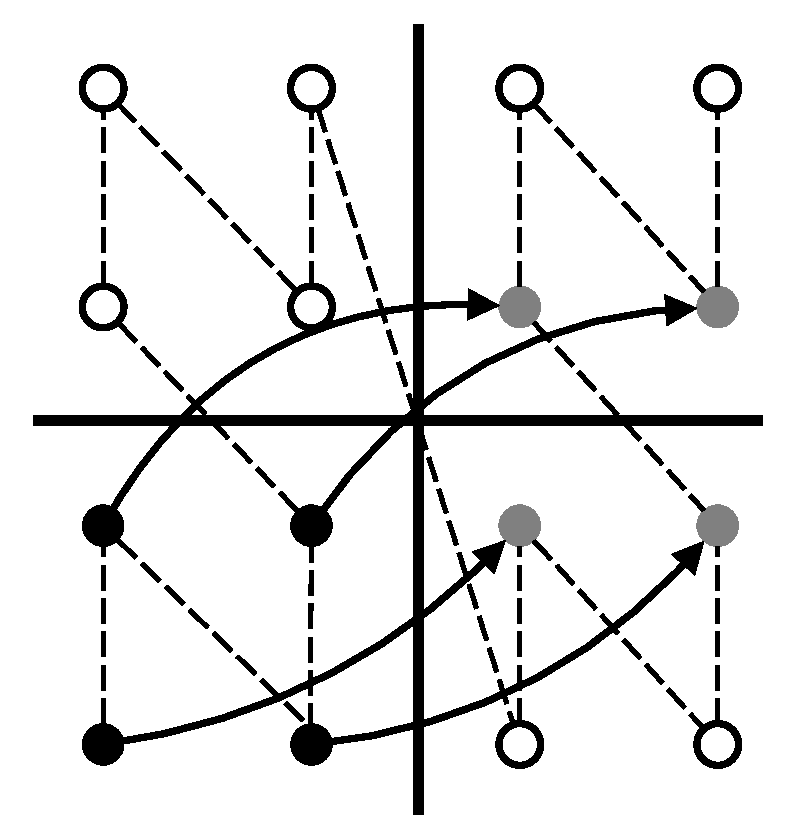
\includegraphics[width=0.5\textwidth]{figures/figure3.pdf}
	\caption{Data shifting.}
	\label{figure3}
\end{figure}

\subsection{Partitioning}
A crucial part of developing a MapReduce application is the way input data are partitioned in order to be delivered to the required reducers. Similar baseline distributed approaches of $k$NN joins problem perform partitioning on both $R$ and $S$ datasets in $n$ blocks each and cross-check for nearest neighbors among all possible pairs, thus requiring $n^2$ reducers. We avoid this issue by computing n overlapping partitioning ranges for both $R$ and $S$, using each element’s SFC values. This way, we make sure that the nearest neighbors of each $R$ partition’s elements will be detected in the corresponding $S$ partition. We calculate these ranges after properly sampling both $R$ and $S$, due to the fact that this process requires costly sorting of the datasets.

\subsection{The FML-\texorpdfstring{$k$}NNN Distributed Processing Framework}
\subsubsection{FML-\texorpdfstring{$k$}NNN workflow}
FML-$k$NN has the same workflow as other similar approaches~\cite{song2015hal}, and consists of three processing stages. The workflow of the algorithm is depicted in Figure~\ref{figure4}. The operations that each stage of FML-$k$NN performs are enumerated below (the Flink operation/transformation is in parentheses):

\begin{itemize}
	\item \textbf{Data pre-processing (stage 1)}:
	\begin{itemize}
		\item Performs dimensionality reduction via SFCs on both $R$ and $S$ datasets (Flat Map $R$/$S$).
		\item Shifts the datasets (Flat Map $R$/$S$).
		\item Unifies the datasets and forwards to the next stage (Union).
		\item Samples the unified dataset (Flat Map Sampling).
		\item Calculates the partitioning ranges and broadcasts them to the next stage (Group Reduce).
	\end{itemize}
	\item \textbf{Data partitioning and organization (stage 2)}:
	\begin{itemize}
		\item Partitions the unified dataset into n partitions, using the received partitioning ranges (Flat Map).
		\item For each partition and each shifted dataset, the $k$NNs of each element in dataset $R$ are calculated (Group Reduce).
	\end{itemize}
	\item \textbf{$k$NN computation (stage 3)}:
	\begin{itemize}
		\item The final $k$NNs for each element in dataset $R$ are calculated and classification or regression is performed (Group Reduce).
	\end{itemize}
\end{itemize}

\begin{figure}[!ht]
	\centering
	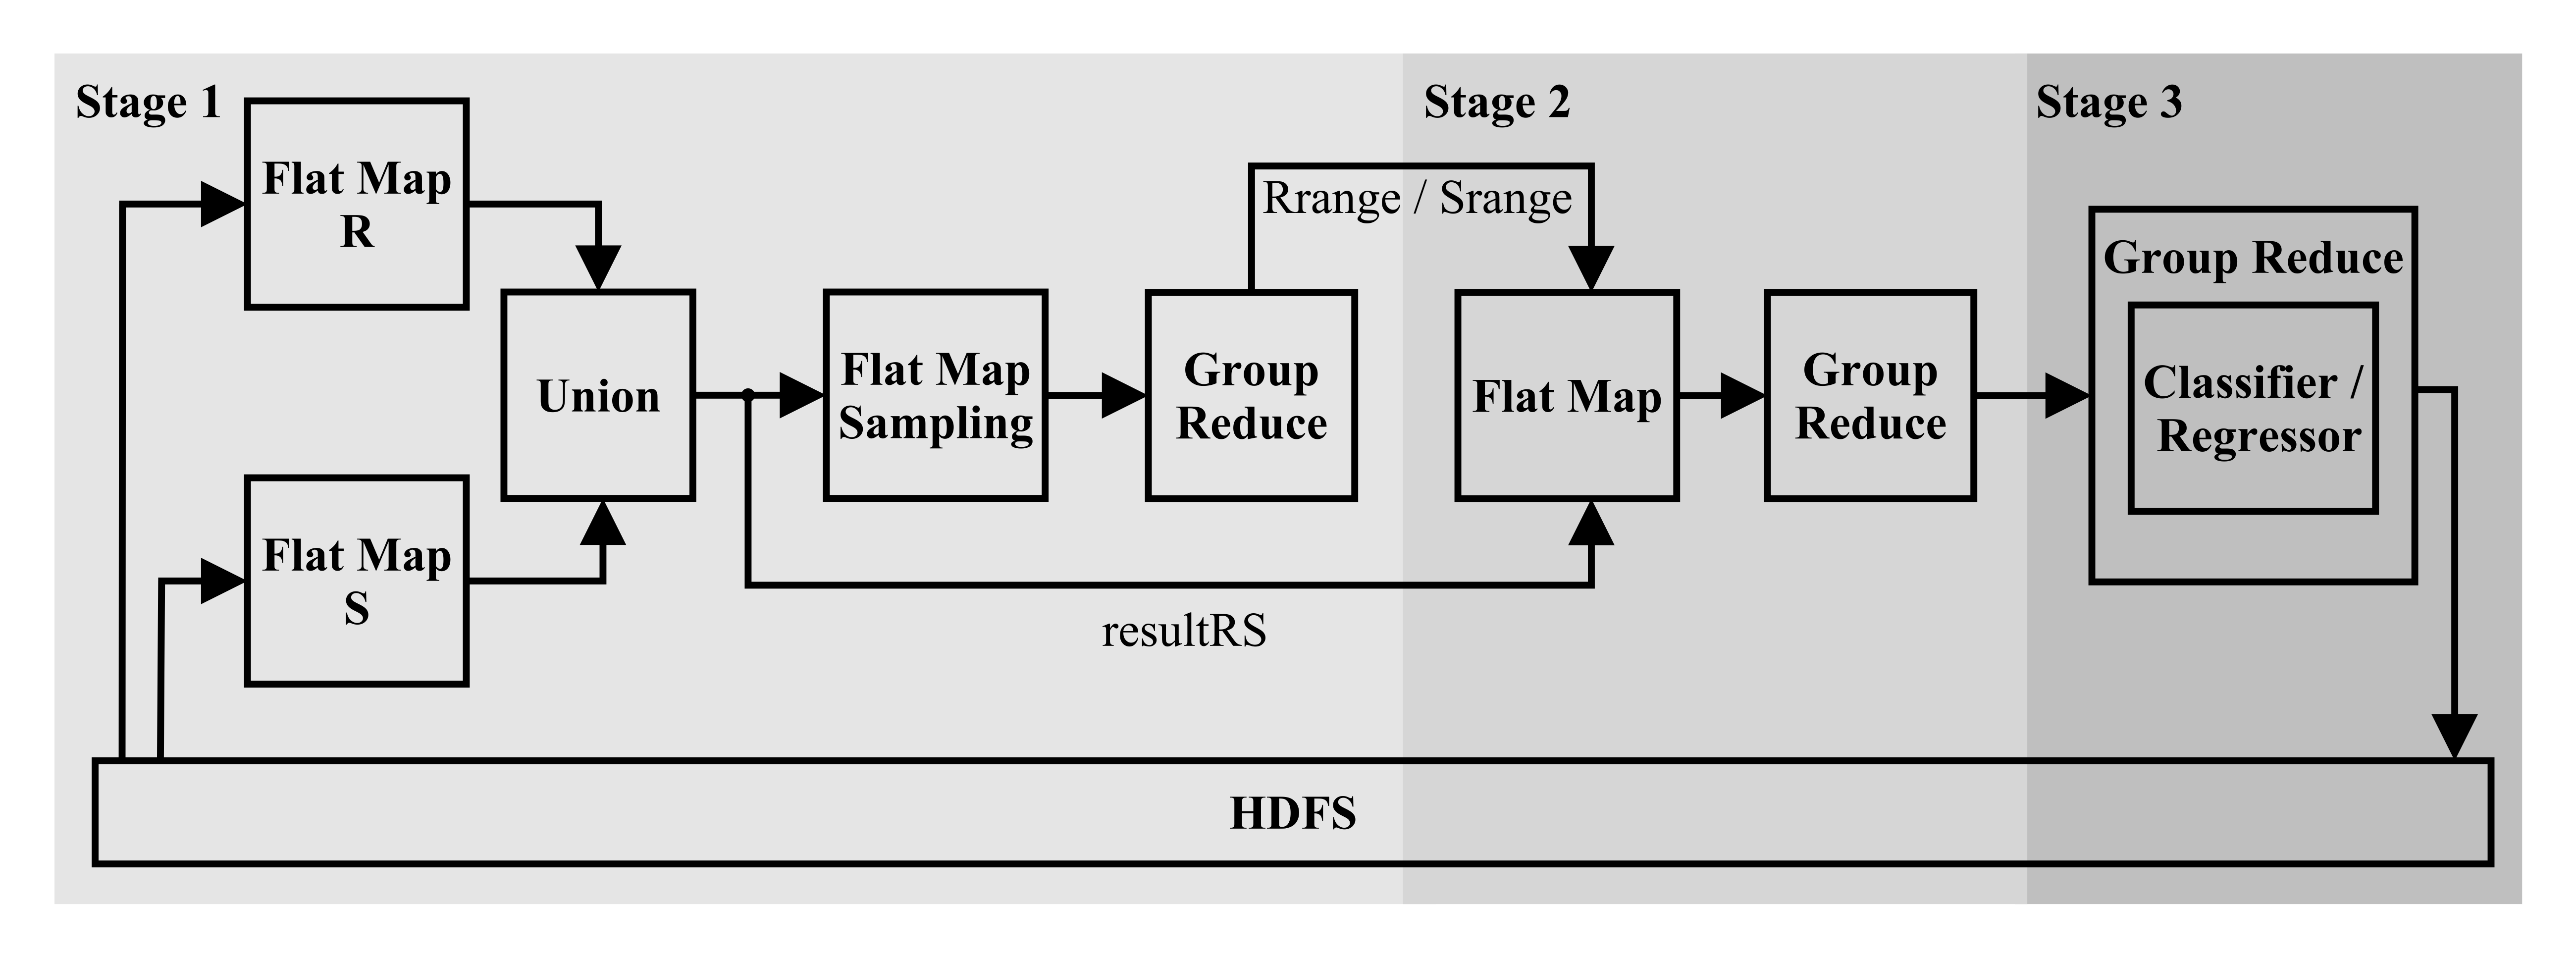
\includegraphics[width=\textwidth]{figures/figure4.png}
	\caption{Single-session FML-$k$NN.}
	\label{figure4}
\end{figure}

During data pre-processing, the sampling process is performed by a separate \texttt{flatMap} operation, which in return feeds the reducers with a smaller, sampled dataset used to calculate the partitioning ranges. The unified transformed datasets are directly passed to the mappers of stage 2, which also receive the partitioning ranges as a broadcast dataset via the \texttt{withBroadCastSet} operation. The data partitioning and organization stage directly feeds the input of the $k$NN computation. Flink's agility allows for the entire removal of the mapping procedure of stage 3, as it only propagates the results from the stage 2 to the reducers of stage 3. This increases the efficiency as it reduces the algorithm's resource requirements. In the following, we present each stage in more details.

\subsubsection{Data pre-processing (stage 1)}
\label{par:algorithmic1}
The $R$ and $S$ datasets are read as plain text from HDFS and delivered to two separate concurrent \texttt{flatMap} transformations, identifiable by the input source file. During this stage, the SFC values ($z$-values for $z$-order, $g$-values for Grey-code curve and $h$-values for Hilbert) and possible shifts, are calculated and passed to a \texttt{union} transformation, which creates a union of the two datasets. The unified and transformed datasets are then forwarded to the next stage (stage 2) and to a sampling process, which is performed by a separate \texttt{flatMap} transformation. The sampled dataset is then passed on a \texttt{groupReduce} transformation, grouped by a shift number. This way, $\alpha$ (number of shifts) reducers will be assigned with the task of calculating the partitioning ranges for $R$ and $S$ datasets, which are then broadcast to the next stage (data partitioning and organization). 

Broadcasting the partitioning ranges significantly reduces the computational resources required by the reducers compared to F-z$k$NN, as it avoids the race condition between stages 1 and 2 (Figure~\ref{figure5}a). During the race condition, the transformed dataset is forwarded to the second stage before the partitioning ranges are calculated by the reducers, causing its mapping operation to be initiated, which would result in an error, as the partitioning ranges are required. To avoid this race condition, F-z$k$NN's reducers have to locally cache the transformed dataset while it is being sampled for the calculation of ranges, as depicted in Figure~\ref{figure5}b. FML-$k$NN overcomes this issue, by broadcasting the partitioning ranges, as this procedure blocks the execution of the second stage until the transformed dataset is ready. The left part of Figure~\ref{figure4} depicts the whole process.

\begin{figure}[!ht]
	\centering
	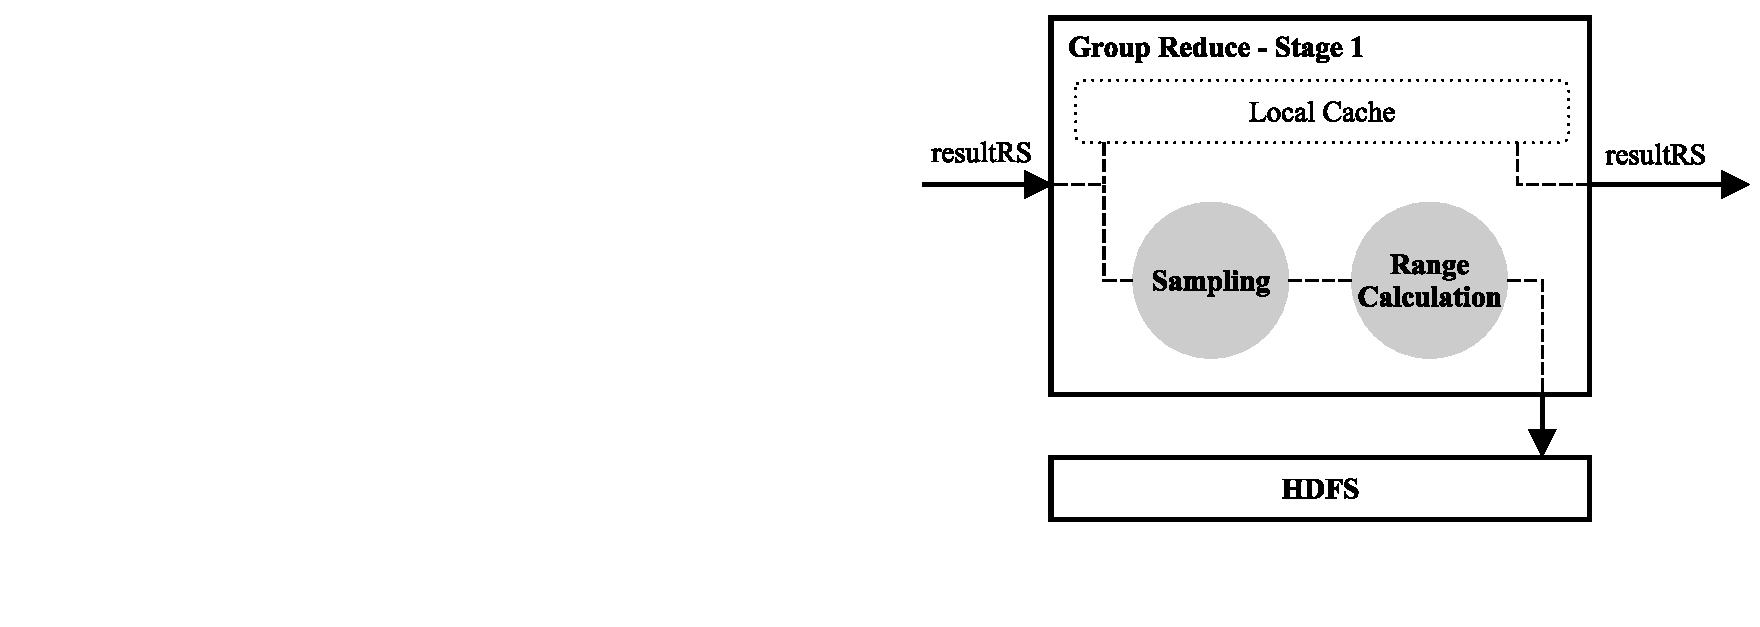
\includegraphics[width=\textwidth]{figures/figure5.pdf}
	\caption{F-z$k$NN race condition and solution.}
	\label{figure5}
\end{figure}

Algorithm~\ref{alg:single_session_algorithm_stage1} presents the pseudocode of stage 1. The random vectors are initially generated and cached on HDFS in order to be accessible by all the nodes which take part in the execution. They are then given as input to the algorithm, along with datasets $R$ and $S$. Notice that $\textbf{v}_1=\overrightarrow{0}$ indicating that the datasets are not shifted during this iteration. This process takes place $\alpha$ times, where $\alpha$  is the number of shifts (Line 5). After shifting the datasets, during the first mapping phase (Lines 5-9), the elements' SFC values are calculated and collected to $\hat{R}^T_i$ and $\hat{S}^T_i$, where $i=1,...,\alpha$. Then, the sampling is performed by the second mapping phase (Lines 10-17). During the reduce phase (Lines 18-22), the partition ranges ($Rrange_i$ and $Srange_i$) for each shift are calculated using the sampled datasets and broadcast to stage 2 (Lines 18-20). The output consists of the unified transformed datasets, which finally feed the data partitioning and organization stage (Line 22).

\begin{algorithm}[!ht]
\begin{small}
	\DontPrintSemicolon
	\Comment The pre-processing stage's input \;
	\KwIn{Datasets $R$, $S$, random vectors $\textbf{V}=\{\textbf{v}_1, ..., \textbf{v}_\alpha\}, \textbf{v}_i=\overrightarrow{0}$ and sampling threshold $\sigma$}
	\Comment The output, that will be emitted to the next stage \;
	\KwOut{Transformed datasets $R^T_i$ and  $S^T_i, i=1,...,\alpha$}
	\BlankLine
	\Begin{
		\Comment The same procedure is repeated for each shift \;
		\For{$i=1,...,\alpha$}{
			$R_i = R + \textbf{v}_i$ \\
			$S_i = S + \textbf{v}_i$ \\
			$R^T_i \leftarrow \proc{calcSFC}(R_i)$ \\
			$S^T_i \leftarrow \proc{calcSFC}(S_i)$ \\
			\ForEach{$x \in R^T_i \cup S^T_i$}{
				\Comment Sampling \;
				$r \leftarrow \proc{Random}(0,1)$\\
				\If{$r < \sigma$}{
					\If{$x \in R_i$}{$\proc{InsertSample}(s, \hat{R}^T_i)$}
					\ElseIf{$x \in S_i$}{$\proc{InsertSample}(s, \hat{S}^T_i)$}					
				}
				
			}
			$Rrange_i  \leftarrow \proc{calcRange}(\hat{R}^T_i)$ \\
			$Srange_i  \leftarrow \proc{calcRange}(\hat{S}^T_i)$ \\
			$\proc{Broadcast}(Rrange_i, Srange_i)$ \\
			\Comment Emit to the partitioning and organization stage \;
			\Return $R^T_i \cup S^T_i$
		}
	}
	\caption{FML-$k$NN (stage 1).}
	\label{alg:single_session_algorithm_stage1}	
\end{small}
\end{algorithm}

\subsubsection{Data partitioning and organization (stage 2)}
\label{par:algorithmic2}
The transformed datasets of stage 1 are partitioned to $n \times \alpha$ blocks via a custom partitioner, after fetching the previously broadcast partitioning ranges. Each block is then delivered to a different reducer through a \texttt{groupBy} operation. Finally, the nearest neighbors for each query element are calculated via proper range search operations and passed on the next stage ($k$NN computation). The middle part of Figure~\ref{figure4} depicts this process.

Algorithm~\ref{alg:single_session_algorithm_stage2} presents the pseudocode of stage 2. During the map phase (Lines 7-18), after having read each shift's broadcast partition ranges (Line 6), the received transformed datasets are partitioned into $n \times \alpha$ buckets ($R^{g \times i}$ and $S^{g \times i}$, $i=1,...,\alpha$, $g=1,...,n$, Lines 13 \& 18), $\alpha$ being the number of shifts and $n$ the number of partitions. The partitions $S^{g \times i}$ are then sorted and emitted to the reducers (Lines 23-30) along with the corresponding partitions $R^{g \times i}$. There, for each $x \in R$ element, a range search is performed on the proper sorted partition in order for its $k$NN to be determined (Line 23) and its initial coordinates are calculated (Line 24). The initial coordinates of all neighboring elements' coordinates are then calculated (Line 26) and their distance to the $x \in R$ element is computed (Line 27). Finally, all nearest neighbors are integrated into the proper dataset ($R_{k \times \alpha}$, Line 28) along with the calculated distance and feed the stage 3, grouped by $x \in R$ elements.

\begin{algorithm}[!ht]
\begin{small}
	\DontPrintSemicolon
	\Comment This stage's input are the datasets emitted during the partitioning and organization stage \;
	\KwIn{Datasets $R^T_i$, $S^T_i$, $i=1,...,\alpha$}
	\Comment The output, that will be emitted to the next stage \;
	\KwOut{Dataset $R_{k \times \alpha}$}
	\BlankLine
	\Begin{
		\Comment Initialization of the dataset to be emitted \;
		$R_{k \times \alpha} = \emptyset$ \\
		$\proc{receiveBroadcast}(Rrange_i, Srange_i)$ \\
		\Comment Again, repeat for each shift \; 
		\For{$i=1,...,\alpha$}{
			\Comment Partition the $R$ elements \;
			\ForEach{$x \in R^T_i$}{
				\For{$g=1,..., n$}{
					\If{$\proc{zval}(s) \in Rrange_i(g) $}{
						$\proc{addintopartition}(s, R^{g \times i})$
					}
				}
			}
			\Comment Partition the $S$ elements \;
			\ForEach{$x \in S^T_i$}{
				\For{$g=1,..., n$}{
					\If{$\proc{zval}(s) \in Srange_i(g) $}{
						$\proc{addintopartition}(s, S^{g \times i})$
					}
				}
			}
			\For{$g=1,..., n$}{
				\Comment Sorting is needed to properly perform range search \;
				$\proc{sort}(S^{g \times i})$ \\
				\ForEach{$x \in R^{g \times i}$}{
					$RES \leftarrow \proc{rangeSearch}(x, k, S^{g \times i})$ \\
					$CC_x \leftarrow \proc{calcCoords}(x)$ \\
					\ForEach{$neighbor \in RES$}{
						$CC_{neighbor} \leftarrow \proc{calcCoords}(neighbor)$ \\
						$CD \leftarrow \proc{calcDist}(CC_x, CC_{neighbor})$ \\
						$R_{k \times \alpha} \leftarrow \proc{add}(x, neighbor, CD)$
					}
				}
			}		
		}
		\Comment Emit to the final stage, grouped by element \;
		\Return $R_{k \times \alpha}$	
	}
	\caption{FML-$k$NN (stage 2).}
	\label{alg:single_session_algorithm_stage2}
\end{small}
\end{algorithm}

\subsubsection{\texorpdfstring{$k$}NNN computation (stage 3)}
\label{par:algorithmic3}
The calculated  $\alpha \times k$-nearest neighbors of each $R$ element, are fetched from HDFS and mapped to $|R|$ reduce tasks. The final $k$-nearest neighbors are determined and passed to the classifier or regressor, depending on user preference. The latter calculate either the probability for each class (classifier) or the final value (regressor) for each element in $R$.

\paragraph{Classification} In the case of classification, we extend the voting scheme, to perform probabilistic classification. We consider the set $P = \{p_{j}\}_{j=1}^{l}$, containing the probability that the query element will belong to each class, where $l$ is the number of classes. The final probability for each class will be derived as follows:

\begin{equation}
	p_{j} = \frac{\sum_{i=1}^{k} w_{i} \cdot I(c_{j} = c_{i}^{NN})}{\sum_{i=1}^{k} w_{i}}, \quad j=1, ..., l
\end{equation}
where $I(c_{j} = c_{i}^{NN})$ is a function which takes the value 1 if the class of the neighbor $x_{i}^{NN}$ is equal to $c_{j}$. 

Finally, the element will be classified as:

\begin{equation} 
	c_{r} = \arg \max_{c_{j}} P, \quad j=1, ...., l
\end{equation}
which is the class with the highest probability. The final result for each element is appended along with the calculated probabilities for each class in a result entry. Listing~\ref{lst:result1} showcases a four class classification where the element XYZ has been assigned to class $C$.

\begin{lstlisting}[caption={The element XYZ is classified to class C, which has the highest probability.}, label={lst:result1}, mathescape=true]
$XYZ | Result: C | A: 0.06 | B: 0.03 | C: 0.71 | D: 0.2$
\end{lstlisting}

\paragraph{Regression} For the case of regression, the final result for each element is calculated as described in Section~\ref{subsec:regression} and contains its predicted value and has the following format (Listing~\ref{lst:result2}):

\begin{lstlisting}[caption={The value estimation of element XYZ.}, label={lst:result2}, mathescape=true]
$XYZ | Result: 19.244469$
\end{lstlisting}

In both cases, the results for each query element are stored on HDFS in plain text.

Algorithm~\ref{alg:single_session_algorithm_stage3} presents the pseudocode of stage 3. During this stage, which consists of only a reduce operation, $k$NNs of each $R$ element are fetched from the grouped set of $R_{k \times \alpha}$. Finally, for each query element either classification (Line 9) or regression (Line 11) is performed, after determining its final nearest neighbors (Line 7). The results are added to the resulting dataset (Line 9), which is then stored on HDFS (Line 12) in the proper format.

\begin{algorithm}[!ht]
\begin{small}
	\DontPrintSemicolon
	\Comment The input is the grouped by element dataset emitted during the previous stage \;
	\KwIn{Datasets $R, R_{k \times \alpha}$}
	\Comment The algorithm's results \;
	\KwOut{Dataset $R_f$}
	\BlankLine
	\Begin{
		\Comment Initialization of the final dataset \;
		$R_f = \emptyset$ \\
		\ForEach{$x \in R$}{
			$RES \leftarrow \proc{kNN}(x, R_{k \times i})$ \\
			\If{$classification$}{
				$FIN \leftarrow \proc{classify}(RES)$	\\
			}
			\ElseIf{$regression$}{
				$FIN \leftarrow \proc{regress}(RES)$	\\
			}
			$R_f \leftarrow \proc{add}(s, FIN)$ \\
		}
		\Comment Store the final results on HDFS \;
		\Return $R_f$
	}
	\caption{FML-$k$NN (stage 3).}
	\label{alg:single_session_algorithm_stage3}
\end{small}
\end{algorithm}

\subsubsection{Spark implementation}
\label{par:spark}
We implemented a three-sessions and a single-session Spark version of the probabilistic classifier, named \textit{S-$k$NN}, in order to conduct a comparative evaluation among the different distributed processing engines. The architecture of the implementation is the same as described above. The main difference lies to the transformations and actions that were used in order to achieve similar functionality to the Flink implementations. The code for both implementations is open source and it can be found online~\cite{daiadAlgs}.

\subsubsection{Cost analysis}
\label{par:cost}
Zhang et al.~\cite{zhang2012epk} showed that the overall communication cost of H-z$k$NN is $O(\alpha(1/\epsilon^2 + |S| + |R| + k|R| + nk))$, where $\alpha$ is the number of shifts, $\epsilon$ the sampling rate, $n$ the number of partitions and $k$ is the number of required nearest neighbors. 

FML-$k$NN introduces some further communication within the stage 1 and between the stage 1 and 2. More specifically, $|R|$ and $|S|$ elements have to be communicated from the initial \texttt{flatMap} of stage 1 to the sampling \texttt{flatMap}. Similarly, the same number of elements have to be sent to the mappers of the stage 2. There is no extra communication from the unification of stage 3, due to the removal of its mappers. Thus, the rest of the communication cost remains unchangeable. Consequently, the overall communication cost of our method is $O(\alpha(1/\epsilon^2 + 3|S| + 3|R| + k|R| + nk))$.

As far as the CPU cost is concerned, Zhang et al.~\cite{zhang2012epk} estimate it to be $O(1/\epsilon^2 log(1/\epsilon^2) + n log(1/\epsilon^2) + (|R| + |S|)log|S|)$ for H-z$k$NN. The FML-$k$NN introduces extra calculations in the stage 3, for classification and regression, which are $O(3k|R| + 2c|R|)$ and $O(2k|R|)$ respectively, where $c$ is the number of classes for classification. However, since both are significantly less than $(|R| + |S|)log|S|$, the total CPU cost is finally equal to $O(1/\epsilon^2 log(1/\epsilon^2) + n log(1/\epsilon^2) + (|R| + |S|)log|S|)$.